\documentclass[a4paper]{article}

\usepackage[margin=1.3in]{geometry}

\usepackage[sc]{mathpazo}
\linespread{1.05}

\usepackage[T1]{fontenc}
\usepackage[utf8]{inputenc}

\usepackage{pdfpages}

\usepackage[francais]{babel}

\usepackage{fancyhdr}
\pagestyle{fancy}

\usepackage{multicol}

\usepackage{color}

\definecolor{gray}{RGB}{106, 106, 106}
\definecolor{dgray}{RGB}{74, 74, 74}

\newcommand{\mytitle}
{\textbf{GConfs}\\Rapport d'activité\\\textsc{S1 (Sept-Dec 2014)}}

\newcommand{\myauthor}
{toogy \textbf{ING1}}

\fancyhf{}
\lhead{\textbf{\thepage}}
\rhead{GConfs -- Rapport d'activité 2014-2015 S1}
\rfoot{\textbf{\thepage}}
\renewcommand{\headrulewidth}{0.4pt}
\renewcommand{\footrulewidth}{0.4pt}

\renewcommand{\labelitemi}{$\bullet$}
\renewcommand{\labelitemii}{$\cdot$}
\renewcommand{\labelitemiii}{$\diamond$}
\renewcommand{\labelitemiv}{$\ast$}

\title{\mytitle}

\author{toogy}

\begin{document}


\maketitle

\section{Conférences}

Liste des conférences organisées par GConfs pendant ce premier semestre :\\

\begin{itemize}
    \item[$\star$] Initiation à Linux\\
        \emph{12 septembre 2014}
        \begin{itemize}
            \item Guillaume \emph{Corwin} Doré
            \item Clément \emph{wxcafe} Hertling
        \end{itemize}
        Linux, Terminal, Shell, man, Vim...ces mots vous évoquent peut-être
        quelque chose sans que vous ne sachiez ce qu'ils veulent vraiment
        dire.
        C'est pourquoi le 12 septembre, GConfs vous présente la conférence
        d'introduction à Linux !
        Lors de cette soirée, deux intervenants vous présenteront les bases
        pour utiliser un système Linux.
        
        Après cette courte conférence se tiendra un TP qui vous permettra de
        mettre en pratique les notions abordées pendant la conférence.
        Des membres de GConfs et des étudiants d'autres promotions seront là
        pour vous assister et répondre à vos questions.
        \vspace{0.3cm}

    \item[$\star$] High Frequency Trading\\
        \emph{13 novembre 2014}
        \begin{itemize}
            \item Julien \emph{Snooze} Lehuen
        \end{itemize}

        Là où la finance et l'informatique fusionnent, quels intérêts pour un
        Épitéen ? Après bientôt deux ans chez IMC Financial Markets, Julien
        Lehuen (EPITA 2013) revient sur son expérience et présente différents
        aspects du travail en tant qu'ingénieur de logiciel financier, quand
        les trades se font par millions et que les latences se mesurent en nano
        secondes. Julien introduira les mécaniques de bases des marchers
        financiers afin de continuer en expliquant le rôle particulier des
        teneurs de marché comme IMC dans ce monde de la finance. Enfin,
        différents projets seront présentés, autour de l'analyse, des
        paramètres ainsi que de l'infrastructure nécessaire au bon
        fonctionnement d'une boite de trading à haute fréquence.

        \vspace{0.3cm}

    \item[$\star$] Facebook Tech Talk\\
        \emph{19 novembre 2014}
        \begin{itemize}
            \item Daniel Bernhardt
        \end{itemize}

        Nous avons le plaisir de vous annoncer qu'un ingénieur de Facebook fait
        le déplacement pour venir faire une conférence avec GConfs à EPITA !\\

        Les sujets abordés seront majoritairement une démystification des
        entretiens à Facebook ainsi que certains de leurs projets internes
        concernant tournant autour du machine learning et de l'administration
        système.\\

        Bonus : un partenariat avec Cook'n'lab et La Paillotte vous permettra
        de pouvoir profiter d'un buffet après la conférence, afin de discuter
        de manière plus détendue avec le conférencier. Deux anciens stagiaires
        de Facebook actuellement en ING3 seront également présents si vous
        désirez un vrai retour d'expérience :)\\

        Venez nous rejoindre le Mercredi 19 Novembre 2014 à 19h30 en Amphi 4 à
        EPITA KB ! Note : De par le contenu un minimum confidentiel de la
        conférence, celle-ci ne sera pas redifusée, ni en live ni plus tard, et
        ce par accord avec Facebook.


        \vspace{0.3cm}

    \item[$\star$] Feedforward Neural Networks\\
        \emph{18 novembre 2014}
        \begin{itemize}
            \item Thibaud \emph{zehir} Michaud
            \item Valentin \emph{toogy} Iovene
        \end{itemize}

        Pour comprendre comment fonctionne réellement un réseau neuronal
        Feed-forward, il faut d'abord s'attarder sur quelques techniques de
        Machine Learning de base et voir que chacune d'entre elles compose en
        fait une brique du fonctionnement interne des réseaux neuronaux. Chaque
        point sera illustré par du code et des exemples (l'exemple de la
        reconnaissance de caractères sera notamment abordé). Nous nous
        attarderons enfin sur l'algorithme de backpropagation et sur les
        optimisations (indispensables) permettant de faire converger votre
        modèle plus précisément et plus rapidement.

        \vspace{0.3cm}

    \item[$\star$] Introduction to C\#\\
        \emph{28 novembre 2014}
        \begin{itemize}
            \item Valentin \emph{toogy} Iovene
            \item Quentin \emph{neodyblue} Coelho
        \end{itemize}

        \vspace{0.3cm}

    \item[$\star$] Bien Démarrer Son Projet\\
        \emph{12 décembre 2014}
        \begin{itemize}
            \item Guillaume Thepau
            \item Quentin Lhours
            \item Sébastien Piat
            \item Alexis \emph{Horgix} Chotard
        \end{itemize}

        \vspace{0.3cm}

    \item[$\star$] Haskell (NDI)
        \begin{itemize}
            \item Kévin \emph{Chewie} Sztern
        \end{itemize}

        \vspace{0.3cm}

    \item[$\star$] Cloud (NDI)
        \begin{itemize}
            \item Kévin \emph{Chewie} Sztern
        \end{itemize}

        \vspace{0.3cm}

    \item[$\star$] Deep Learning (NDI)
        \begin{itemize}
            \item Quentin \emph{underflow} de Laroussilhe
        \end{itemize}

        \vspace{0.3cm}

    \item[$\star$] Fact (NDI)
        \begin{itemize}
            \item Raphaël \emph{Shugo} Boissel
        \end{itemize}

        \vspace{0.3cm}

    \item[$\star$] Live Photoshop
        \begin{itemize}
            \item Meven \emph{mevouc} Courouble
        \end{itemize}

        \vspace{0.3cm}

    \item[$\star$] OpenGL (NDI)
        \begin{itemize}
            \item Raphaël \emph{Shugo} Boissel
        \end{itemize}

        \vspace{0.3cm}

    \item[$\star$] From native to JIT (NDI)
        \begin{itemize}
            \item Guillaume \emph{Vermeille} Sanchez
        \end{itemize}

        \vspace{0.3cm}

    \item[$\star$] Keep Calm And Blame The Algorithm (NDI)
        \begin{itemize}
            \item Jill-Jenn Vie
        \end{itemize}

        \vspace{0.3cm}

    \item[$\star$] How to Kill A Bison With A Menhir (NDI)
        \begin{itemize}
            \item Valentin \emph{nitnelave} Tolmer
        \end{itemize}

        \vspace{0.3cm}

    \item[$\star$] KikooC++ \& Goto++ (NDI)
        \begin{itemize}
            \item Guillaume \emph{Vermeille} Sanchez
            \item Alexis \emph{Horgix} Chotard
        \end{itemize}

        \vspace{0.3cm}
\end{itemize}

\section{Partenariats}

\subsection{Présentation des projets de SUP}

Chaque année GConfs organise la présentation des projets de jeux-vidéo par les
SPE aux SUP.

\subsection{JDMI}

L'association continue d'organiser les ateliers de programmation pour les
lycéens pendant les JDMI. Il est cependant parfois difficile de trouver des
membres disponibles pour le faire.

\subsection{Assistants}

À l'occasion de certaines conférences, \emph{GConfs} organise également des TP
(exercices de programmation) pour que les spectateurs puissent appliquer ce
qu'ils viennent d'apprendre (\emph{In theory, theory and practice are the same.
In practice, they’re not.}).

\subsection{JPO}

L'association est présente à toutes les JPO EPITA et EPITECH.

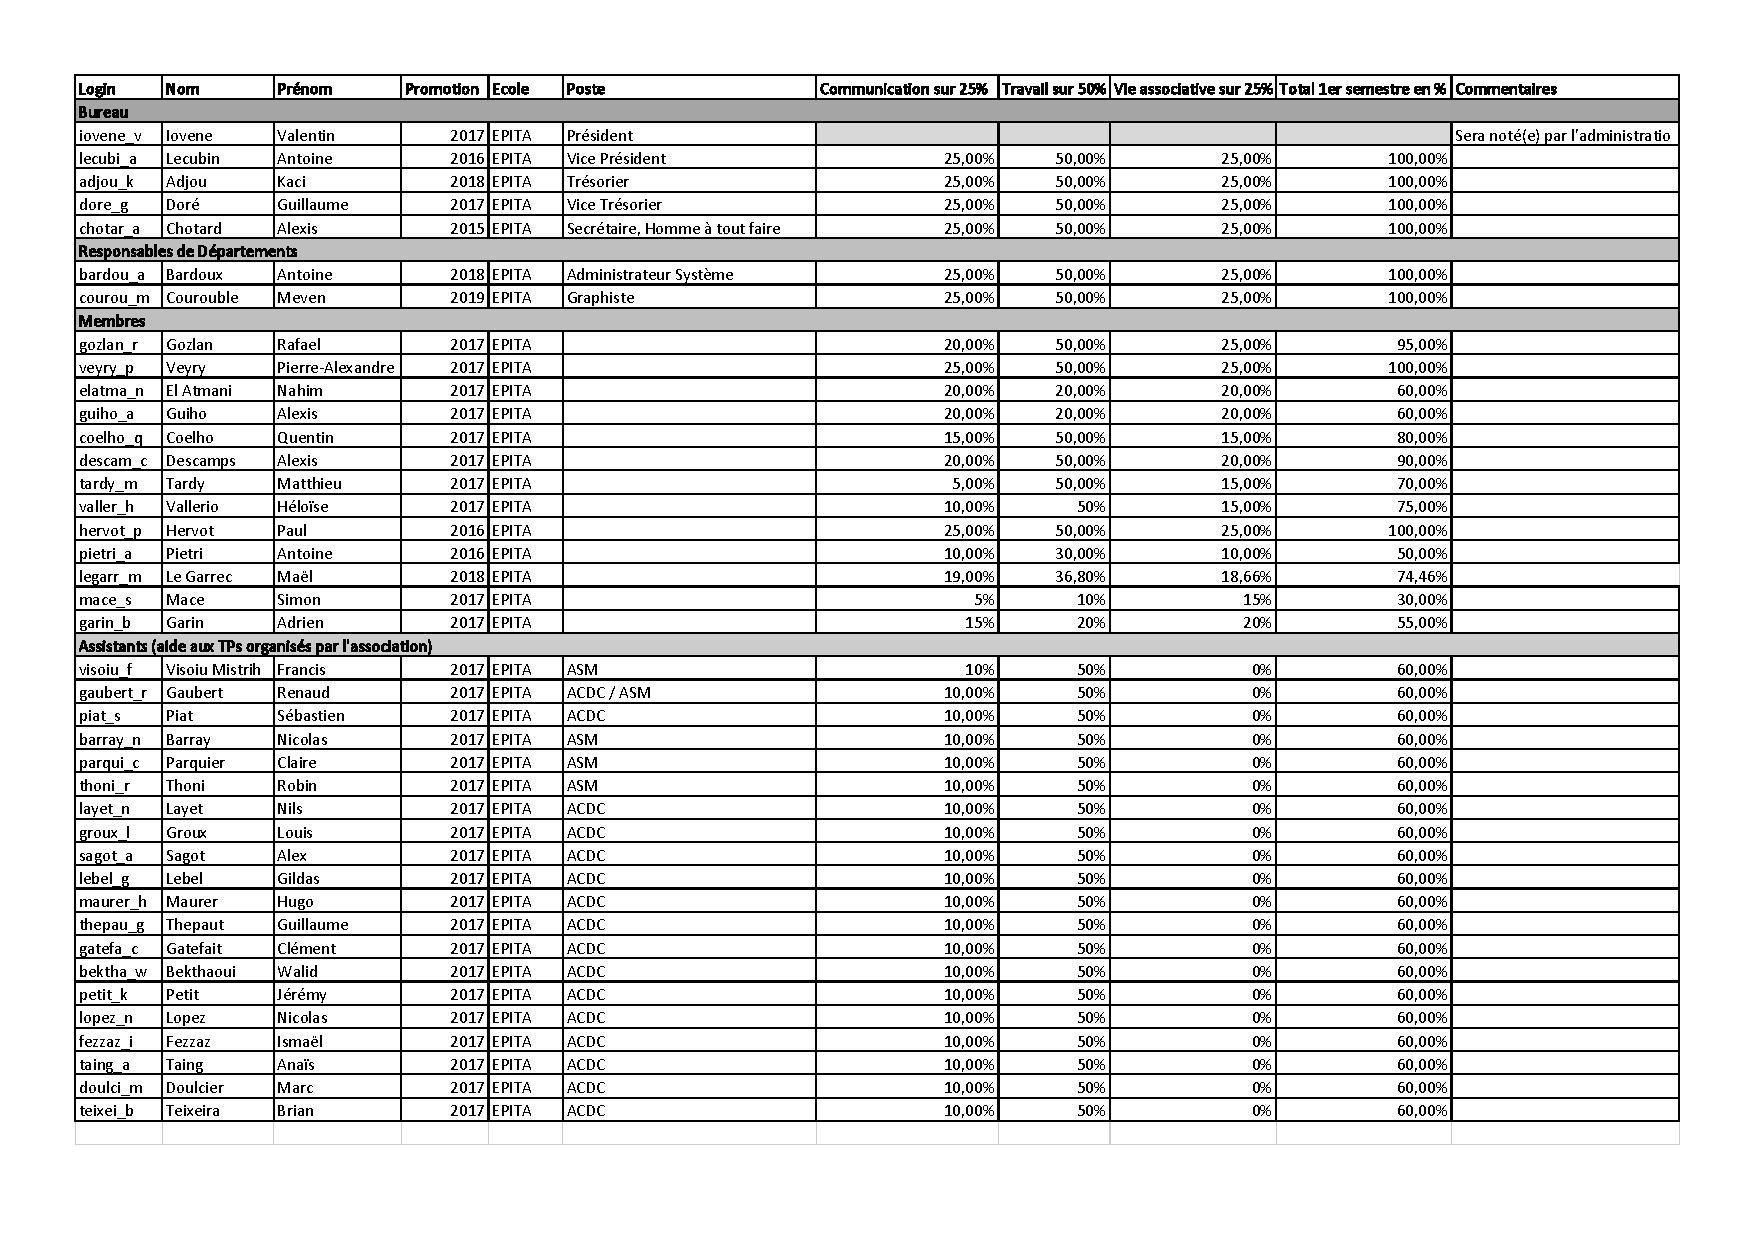
\includepdf{enac.pdf}

\end{document}

